	
\documentclass[12pt]{article}
\usepackage{geometry} % see geometry.pdf on how to lay out the page. There's lots.
\geometry{a4paper} % or letter or a5paper or ... etc
% \geometry{landscape} % rotated page geometry
\usepackage{url}
\usepackage{graphicx}
\usepackage{placeins}
\usepackage{amsmath}

\newcommand{\code}[1]{{\fontfamily{phv}\selectfont \small{\begin{tabbing} #1 \end{tabbing}}}}

\title{Natural Language Programming Analysis in Scala}
\author{\\ \'Eric Zbinden \\ \texttt{eric.zbinden@epfl.ch} \\ \\ Supervisors: \\Philippe Sutter(\texttt{philippe.sutter@epfl.ch})\\ Philipp Haller(\texttt{philipp.haller@epfl.ch})\\Prof. Viktor Kuncak(\texttt{viktor.kuncak@epfl.ch}) \\ \\ EPFL\\ Laboratory for Automated Reasoning and Analysis (LARA) \\ \url{http://lara.epfl.ch/}\\ Programming Methods Laboratory (LAMP) \\ \url{http://lamp.epfl.ch/} }
\date{\today}

\begin{document}

\maketitle
\newpage
\tableofcontents
\newpage

\section{Introduction}
The lexical analysis of programming language is growing in interest. Researchers are more and more interested in this topic, as is the industry. A program written in a complex language without proper explanation will cause trouble to be understood by everybody. That could be quickly becoming a problem inside a team project or during a presentation of a product to a client that know anything to programming. This is where is the matter to name methods and variables with a comprehensible, useful and meaningful name.  H{\o}st and {\O}stvold in their paper \textit{Debugging method names}~\cite{DebugMN} looked at grammatical syntax and abstract phrasing of method names in Java programs to discover naming bugs.

\section {Project Overview}
The main idea of this project is to apply an analysis similar to H{\o}st and {\O}stvold~\cite{DebugMN} but to the Scala language. As Scala is a functional object-oriented language it contains possibilities that Java don't contains. So I tried to focus on theses particularities as much as possible. The analysis done during this project will very few focus on phrasing but will focus in finding inconsistencies inside method declarations.\\

This was a challenging project as I didn't know what I will find out, if off course there is something to find out.
I worked on a Windows XP platform, which added some additional difficulties. Nothing impossible to face off, but it cost sometimes valuable time. Working with the Scala compiler was a great opportunity to improve my knowledge of Scala and to see the language evolving. When I asked some specific questions, where I was guided to a particular class or package of the compiler, sometimes that class or package was modified or removed just a few days before. My programming experience coming mostly from Java, I had the assumption that Scala was kinda similar to Java and therefore would behave the same way for some features. Well, I can say that I revised completely my assumptions. 
\newpage
\section {Implementation}
For analyzing a program, the first thing to do is to retrieve information about it. The best way is to create an extension plug-in of the Scala compiler and let it collect every things we want.

\subsection{Compiler plug-in}
My plug-in, named \textit{Scala-names}, is inserted into the compiler phases right after phase 7:~\textit{refchecks}. It use the abstract syntax tree produced in previous phases to extract all objects named by the programmer. It could be variables names, objects names, methods names, parameters names or types names. It perform an analysis and then kill the resting compiler phases, as we don't need them for the analysis.\\

By lack of time, the analysis is run only on method names. But the plug-in could easily be improved to also analyze other objects.
The plug-in check for every method declarations found in the given files, if theses methods match features. See~\ref{features} for more details on features. The plug-in output for every method declarations found a list of 1 or 0 depending on this method satisfy or not a feature and the method name with source and position. See here an example of the output of the plug-in:
\code{1 1 0 0 0 0 1 1 0 0 0 0 0 0 0 1 1 0 0 1 0 0 0 0 1 0 0 0 0 0 0 0 0 1 0 0 0 0 0 \\empty@source-scala$\backslash$collection$\backslash$Map.scala,line-30,offset=1212}
You can see in the first line if the method, here \textit{empty} of the trait \textit{Map} defined in the \textit{scala$\backslash$collection$\backslash$Map.scala} file at line 30, match the features implemented inside the plug-in.
\subsection{Features}
\label{features}
A feature is a boolean property that a method may satisfy or not. I tried to implement all the features that H{\o}st and {\O}stvold~\cite{DebugMN} used. I added features proper to the Scala language. Then I search into the \textit{Symbol} class given by the Scala compiler and implemented what I thought to be interesting and possible. Here is a list of features that I implemented:

\begin{enumerate}
\item ReturnTypeCOLLECTION :\\
	The return type is a collection. To be enough general to match a return of a List, a Set or a Map, it's implemented to match any class that extends the Traversable trait~\cite{travers}.
\item ReturnTypeOBJECT : \\
	This feature match any return type that extends the AnyRef class~\cite{anyRef}.
\item ReturnTypeUNIT :\\
	This feature match if the return type is Unit.
\item ReturnTypeBOOL : \label{fBool}\\
	Straight forward, this feature match boolean return type.
\item ReturnTypeINT :\label{fInt}\\
	Same as feature~\ref{fBool} with Integer return type.
\item ReturnTypeSTRING : \\
	Same as features~\ref{fBool} and~\ref{fInt} with String return type.
\item HasNoParameters :\label{fNoParam}\\
	This method is a variant of feature~\ref{fNoParenthesis}, see it for more details.
\item HasNoParenthesis :\label{fNoParenthesis}\\
In Scala when a programmer declare a function that take no argument, it's possible to write with or without parenthesis. With parenthesis indicate by convention that this function have side effect; modifying data, printing out on std. In the abstract syntax tree produced by the compiler, the parameters of a method are returned as a List of Lists. If the first list is empty, then it indicate that this method is declared without parameters and no parenthesis and should therefore have no side-effect. If the first list is of size one and contains an empty list, we have here a method declared without parameters but with parenthesis and thus with possible side-effect. And if the first list have a bigger size than one, it indicate we are dealing with a currified function.
\item ContainsIF :\\
	The method body contain an IF branch. Note that the Scala compiler translate WHILE block and DO-WHILE block with a IF branch. These two cases should not match this feature as the programmer did not write any IF branch. IF guard statement in pattern matching are not taken in account as IF branch. However an IF branch inside a pattern matching right hand side will match. See here an example:\\ \\
\begin{minipage}{8cm}
IF branch inside pattern matching:
\code{
ls \=match \{\\
\>case Nil =$>$\ false\\
\>case x\ ::\ xs =$>$\ if(x==0) true else false\\
\}\\
}
\end{minipage}
\begin{minipage}{10cm}
IF guard:
\code{
ls \=match \{\\
\>case Nil =$>$\ false\\
\>case x\ ::\ xs if(x==0) =$>$\ true\\
\>case x\ ::\ xs =$>$ false\\
\}
}\end{minipage}
\item ContainsWHILE :\\
	The method body contains a WHILE statement. DO-WHILE statement are also considered as WHILE statement.
\item ContainsTRY-CATCH :\\
	The method body contains a TRY-CATCH block. If a method body contains only the TRY block, it will also match.
\item ContainsPatternMatching :\label{fPatternMatching} \\
	The method body contains pattern matching. This feature match if the method body contains a MATCH statement.
\item ThrowException :\\
	The method body contains a THROW statement. It match only if it's explicitly declared. By example, A NumberFormatException raised by a wrong string applied to \textit{.toInt} will not match.
\item IsCurrified : \\
	This feature is a variant of feature~\ref{fNoParenthesis}. See it for more details.
\item IsSelfRecursif : \\
	This method call it-self in it's body. The feature don't match for others methods with surcharged identifiers. If a method call another method that call back the first method, it will not be considered as self-recursive.
\item MethodNameIsVerb : \label{fVerb}\\
	This feature match if the method name is a verb. It could be an infinitive or a conjugated form. For this feature, it use the WordNet 2.1 database~\cite{wordNet} to determine it.
\item MethodNameIsNoun :\\
	This feature match is the method name is a noun. It could be a singular form or a plural. As in feature~\ref{fVerb}, it use also the WordNet 2.1 database~\cite{wordNet}.
\item CamelPhrase : \label{fCamel}\\
	A unique word is not always meaningful to name a method. As C convention use underscore-separated words like \textit{end\_of\_file}, Java and Scala convention use camel case. Camel case is a practice of writing several words composed without white space but with the first letter of each word in uppercase. The first letter of the first word may or not be in uppercase.\\
This feature split the method name by the non-letter characters and by uppercase letters. Then it reconstruct potential acronym like in feature~\ref{fAcronym}. Then the feature will match if the split is composed at least of two words and if the second and followings words begin with an uppercase letter. Example:
\code{aCamel++Case\_PhraseWithXML \= =$>$ List(a, Camel, Case, Phrase, With, X, M, L)\\
\>=$>$ List(a, Camel, Case, Phrase, With, XML)\\
\>=$>$ true
}
Note that \textit{an\_Underscore\_Separated\_Phrase} will match this feature as all words, except the first, begin with an uppercase letter.
\item ContainsAcronym :\label{fAcronym}\\
	An acronym is defined by the aggregation of uppercase letters and digits. It must start with a letter. Non-letter nor digit characters are considered, as in feature~\ref{fCamel}, as blank and thus discarded. Inside a camel case phrase, the acronym is construct correctly: the acronym inside \textit{XMLAsString} is reconstruct as \textit{XML}. But as the underscore will also considered as a blank, two acronyms separated by an underscore will create one acronym instead of two.\\
This feature will match if the method name contains at least one word that is an acronym.
\item MatchAbstractPhrase :\label{fAbstractPhrase} \\
	The method name is split the same manner as feature~\ref{fCamel} and if it contains the words \textit{get}, \textit{set}, \textit{contains} the next word should be a noun or an acronym. If the method name contains the word \textit{is} it should be followed by an adjective or an acronym. Acronyms are defined in feature~\ref{fAcronym}. To find out if the following word is an adjective or a noun, it use the WordNet 2.1 database~\cite{wordNet}. Like in feature~\ref{fContainsIs}, theses words can be written with a capital letter or without. If the method name don't contains theses four words, this feature return trivially true. This feature will also match on operators. See operators in feature~\ref{fOperator}.
\item ContainsWordIS :\label{fContainsIs}\\
	As in features~\ref{fCamel} and~\ref{fAcronym}, the method name is split into words. Then if at least one word is \textit{is}, then the feature will match. \textit{is} can be written \textit{is} or \textit{Is}.
\item ContainsWordGET :\label{fContainsGet}\\
	Straight forward, it's implemented the same way as feature~\ref{fContainsIs}.
\item ContainsWordSET :\label{fContainsSet}\\
	Same as features~\ref{fContainsIs} and~\ref{fContainsGet}.
\item ContainsWordCONTAINS :\label{fContainsContains}\\
	Same as features~\ref{fContainsIs},~\ref{fContainsGet} and~\ref{fContainsSet}.
\item IsValidJavaName :\label{fValidJavaName}\\
	A valid Java method name is a series of Java letters or Java digit that begin with a Java letter~\cite{jls_ident} and that is not a Java keyword~\cite{jls_keyword}. However as the Scala library is developed in English, for simplicity, it only take in count as letter Latin characters without accent.
\item IsOperator :\label{fOperator}\\
	An operator is defined as a following of characters that are neither a letter neither a digit. This feature will match if the method name is an operator.
\item ReturnTypeCompletelyInMethodName :\label{fReturnTypeComplete}\\
	This feature match if the return type is contained into the method name. For composed return type name, the method name should match for every words in the correct order. The return type name and the method name are split the same manner as in feature~\ref{fCamel}. 
\item ReturnTypePartiallyInMethodName :\\
	This feature is a variant of feature~\ref{fReturnTypeComplete}. For composed type name, as programmer are often lazy, they often write it partially. One would by example write only \textit{Tree} instead of \textit{AbstractSyntaxTree}.
\\This feature will match if the method name contains partially the return type name. It will also match if the type is completely contained, like in~\ref{fReturnTypeComplete}.
\item RightAssociative :\\
	Scala language is left associative. But a method name that finish with the \textit{:} character is right associative.
%ajouter qqch ici
\code{
1\ ::\ List(2, 3) \==$>$ List(2, 3)::.(1)\\
\>=$>$ List(1, 2, 3)
}
This feature match if the last character of the method name is \textit{:}\ .
\item InnerMethod :\label{fInner}\\
	Scala language allow declaration of functions inside function. It's a good way to declare subroutine that should not be used outside of this function.\\
This feature match if the method body contains a method declaration.
\item ContainsInnerMethod :\\
	This feature is the opposite of feature~\ref{fInner} and match if the method body contains a method declaration.
\item Override : \\
	This feature match if this method override another method.
\item IsAbstract :\\
	This feature match if the method body is empty.
\item IsPublic  :\label{fPublic}\\
	A method declared public inside an object can be called from outside of that object. Note that inner function are always public by language specification but can't be accessed from outside.\\
This feature match if this method is public.
\item IsStatic :\\
	A static method can be called without having an object where the method is declared.\\
This feature match if this method is static. 
\item MethodNameFinishWithS :\label{fs}\\
	It's a naming convention that a method name finishing with a \textit{s} have a collection as return type.\\
This feature match if the last character of the method name is \textit{s}.
\item MethodNameFinishWithSS : \label{fss} \\
	Similar to feature~\ref{fs}, a method name finishing with \textit{ss} would mean this method return a collection of collections.\\ 
	This feature match if the two last characters of the method name are both~\textit{s}.
\item ContainsLazyVal :\\
	This feature match if the method body contains a lazy val.
\item IsImplicit : \\
	This feature match if the method is declared implicit.

\end{enumerate}
\subsection{Clustering}
\label{cluster}
With the output of the Scala-names plug-in, I filled the \textit{k}-means algorithm~\cite{kMeans}. %hoping the result will be interesting.
The implementation of the algorithm follow~\cite{kMeans} description with a random partition. The distance between two methods is calculated as:
\begin{equation}
d_{m1\_m2} = \sum_i{ |m1_{f_i}-m2_{f_i}|}
\end{equation}
With $f_i$ equals to 1 if feature $i$ match or otherwise 0. \textit{K}-means is sensible to the initial partitioning and its output may be different. The output may also contains empty clusters. As \textit{k}-means reach a stable point fast, it's generally recommended to run several times the algorithm to be sure to obtain a fine result.\\

First question, how many clusters should we use? A too small number of clusters will aggregate different groups of methods and a too high number of clusters will separate similar methods. The answer to this question really depend on the data set and what we want to find out. This cluster model is a key limitation of the algorithm. It's concept is based on spherical clusters expected of similar size. Therefore the choice of the number of clusters is critical. See~\ref{cluster:exp} for an answer based on this project.\\

At the end of the algorithm, we obtain clustered data. Fine, but the center of cluster is a raw position, as it's the average position of all its members. To obtain a position more readable an more meaningful, I discrete the position of the clusters depending on a threshold to obtain a position only composed of: $0$, $1$ or $?$. If for a given dimension the value is lower than the threshold, the value is lowered to $0$. Respectively if the value is higher than $1-threshold$, the value is raised to $1$. And if the value is higher than \textit{threshold} and lower than $1-threshold$, the value is set to undefined, noted with a \textit{?}. See figure~\ref{discrete} for an example on two dimensions. Then I restart \textit{k}-means with theses discrete clusters. During the project I was running only one-step of the algorithm with discrete clusters, thinking it would not converge. This was at first to check the effect of the discretization to the clusters, but as it seams to converge, I took this advantage to get a better clustering. During this second run the distance of a method to a cluster is defined this way:
\begin{equation}\label{equa1}
d_{m\_c} =\mbox{if} (n-m ==0) \mbox{\scriptsize{ Double.MAXVALUE }\normalsize{ else }}\frac{n*\sum_{i: g_i\ defined} |m_{f_i}-c_{g_i}|}{n-m}
\end{equation}
With $n$ the dimension of the cluster (i.e. the number of features, here 39), $m$ the number of undefined values of this cluster, $f_i$ equals to 1 if this method match feature $i$ otherwise 0, and $g_i$ the value of the position of the cluster at the $i^{th}$ feature for a defined value. Note that a completely undefined cluster would raise a division by zero and would learn us anything, thus it's distance is considered to be the maximum value to move members of this cluster to a more appropriate cluster.\\

Here, another question is raised: what's a relevant threshold? It should be small enough to minimize the amount of methods that move to another cluster during the second \textit{k}-means run, but big enough to have a minimum of undefined values. See the respond in section~\ref{threshold}.
\begin{figure}[tbc]
\centering
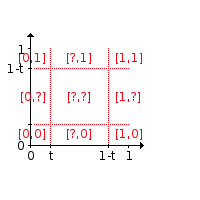
\includegraphics[width=5cm]{images/discrete.png}
\caption{Discretization of a cluster of two dimensions depending on it's position}
\label{discrete}
\end{figure}
\subsection{Analysis}
\label{analysis}
By giving the option \textit{pAnalysis} to the plug-in, it's possible to analysis files compared to the Scala library. It's possible to pass several files with this option, but as the output of this option is quite long, it's recommended to pass only one file in argument. Like in previous points, it collect all method declarations. Then for every method declarations, it check all the 39 features and output a complete user friendly analysis. This analysis is done based on an already computed \textit{k}-means algorithm result of an analysis of the Scala library.\\
The result of the plug-in analysis contains for all method declarations, a signature based on the 39 features, the nearest cluster with it's distance, three methods from the Scala library took at random from the same cluster and for all features a line saying if this method match the feature or not, referred to the three random selected methods and to it's belonging cluster. If the method declaration is different to it's cluster, it will be noted. If the cluster is undefined for this feature, it output three dots. See an example of the output in annexes~\ref{annexe1}.
\section {Experimental Results}

\subsection {Clustering}
\label{cluster:exp}
To answers the two questions of section~\ref{cluster}, I ran 100 times the \textit{k}-means algorithm on the output of the Scala-names plug-in of the Scala library with different numbers of clusters. I took five mean metrics with confidence interval of 95\%: the number of empty clusters, the number of undefined values in all clusters, the average distance of methods to their respective cluster, the cluster average size and the error due to discretization modeled by the number of methods moving after a one-step of the second \textit{k}-means. 
\subsubsection{Number of clusters}
For this series of experiments, the threshold was fixed at 0,15. 
\\
\begin{center}
\begin{tabular}{c c}
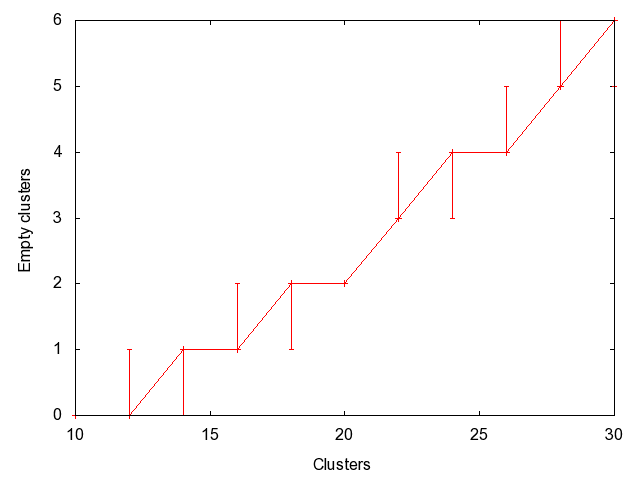
\includegraphics[width=5cm]{images/emptyCluster.png}
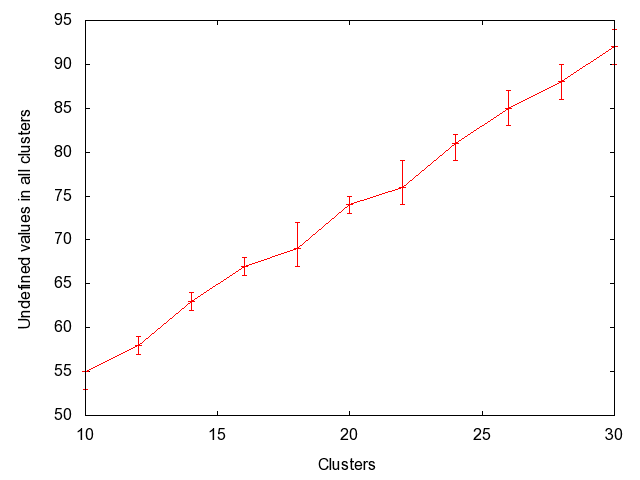
\includegraphics[width=5cm]{images/questionMark.png}
\end{tabular}\\
\begin{tabular}{c c c}
\hspace*{-0,5cm}
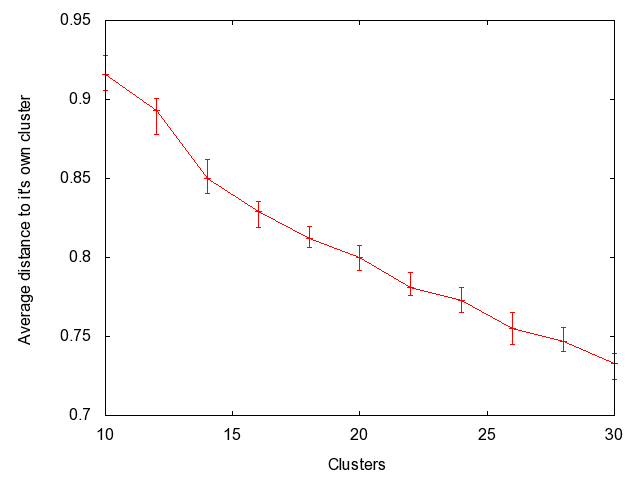
\includegraphics[width=5cm]{images/averageDist.png}
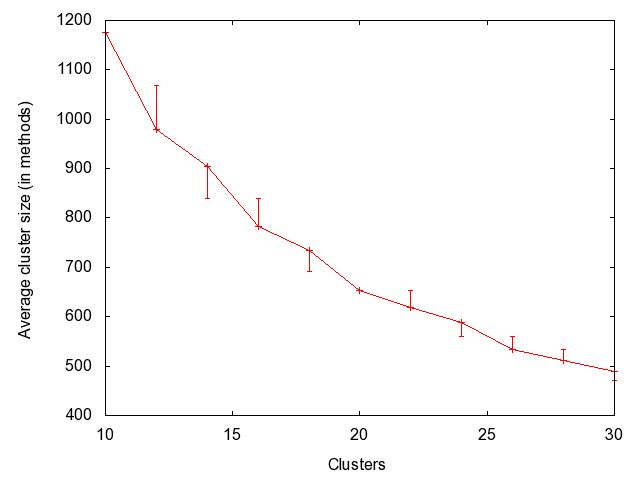
\includegraphics[width=5cm]{images/averageClusterSize.png}
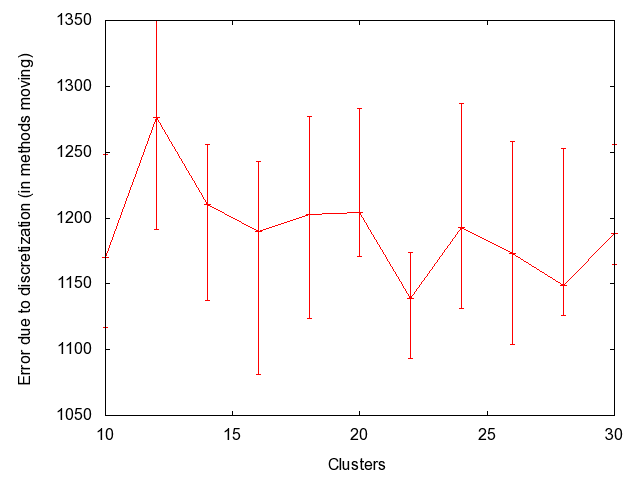
\includegraphics[width=5cm]{images/switched.png}
\end{tabular}
\end{center}

\begin{enumerate}
\item As the number of clusters increase, the number of empty clusters increase too. With 30 clusters we reach 6 empty clusters. It represent a percentage of empty clusters of 20\%, which is pretty high. There is no point to compute a clustering algorithm with a lot of clusters if they all finish empty. As The computational time of the algorithm also increase with a higher number of clusters, it suggest that a lower number of clusters is better.
\item To be independent of the first metric, the second it is calculated only with non-empty cluster. The number of undefined values in the clusters also increase with the number of clusters on a linear basis. This is bad as we can't deduce anything from an undefined value. So it tend to say here again, a low number of clusters gives better results.
\item The third metric doesn't answer our question. If the distance of a method to it's own cluster decrease, that's good, as the cluster is a better representation of its members. But as the result for 10 clusters is already below a distance of one, a so small difference have no impact.
\item As the fourth metric show the average cluster size, we can pretend that a cluster with a smaller number of members will be more accurate. My experience on this project would say the same, as during the development of the project I get as a first result of \textit{k}-means, with 10 clusters, a pretty strange result: as all the 10 clusters have a negative result for the feature~\ref{fPatternMatching} \textit{ContainsPatternMatching}, I looked into some files at random, saw that it were true for those files and stated: "\textit{Yes, that's true, the Scala library do not contains any pattern matching.}" Off course, that's wrong. But pattern matching is found only in 8\% of all methods, making this feature less representative than feature with a higher probability. A small number of clusters will hide results on some features. %On the other hand, as pointed by the second metric, the number of undefined values increase which try to say that to obtain a smaller granularity we need to cut some concentrated points.
\item The last metric seams unstable and really depend on the initial partitioning. But we need to consider the library size: 11'753 method declarations. The variation of the mean is of 1\% and the number of methods that move to another cluster stay on a percentage of 10\% of all methods. I noted that this percentage of moving methods was lower with a lower cluster dimension (i.e. less features). We can conclude that the number of clusters don't impact on the error due to discretization.
\end{enumerate}
On the basis of theses results, I decided to take a number of clusters of 15 to shrink the cluster size at maximum without to suffer of bad effects of undefined values.
\subsubsection{Threshold}
\label{threshold}
Here again, I ran 100 times the same experience, but this time with a fixed number of clusters of 15, on different thresholds. I choose the five same metrics. The number of empty clusters and the average cluster size are not represented here because they were constant. For every measures it return only one empty cluster and an average cluster size of 839,5 methods.
\begin{center}
\begin{tabular}{c c c}
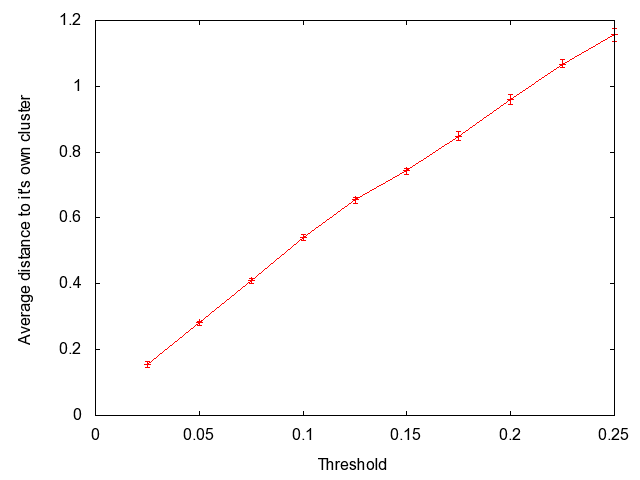
\includegraphics[width=5cm]{images/taverageDist.png}
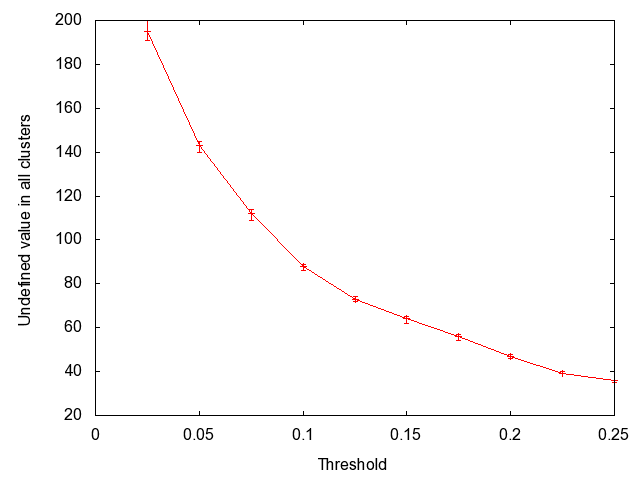
\includegraphics[width=5cm]{images/tquestionMark.png}
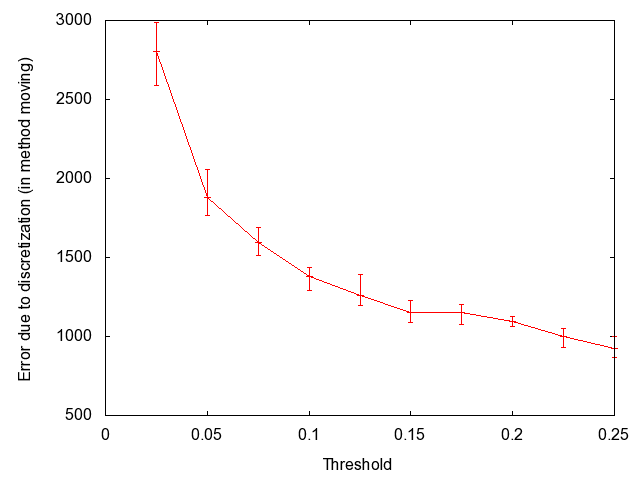
\includegraphics[width=5cm]{images/tswitch.png}
\end{tabular}
\end{center}
\begin{enumerate}
\item The average distance increase linearly with the threshold. The line cross a distance of 1 near a threshold of 0,2125. This distance depend on undefined values as the distance is normalized on them. For the same threshold, we have about 40 undefined values. So from equation~\ref{equa1} we can reconstruct~the~distance:\begin{align*}
1 &=\frac{n*d}{n-m}\\
d &= \frac{n-\frac{m}{c}}{n}
\end{align*} With $c$, the number of clusters fixed to 15 and $n$, the dimension of the clusters fixed to 39 (i.e. the number of features). We obtain:\begin{align}\label{equa2}
d = \frac{39-\frac{40}{15}}{39} = 0,9333
\end{align}
Equation~\ref{equa2} mean that the cluster represent correctly it's members with an error of $\pm$1 feature or an average error of $\pm0,02$ per feature.\\ Note that I didn't test with a threshold of zero. I expected a such experience finishing with all clusters being filled only with undefined values.
\item As expected, the number of undefined values decrease as the threshold increase. This is a major criteria to obtain meaningful results, so choosing a high threshold is really important. From this metric point of view, it could be interesting to test with a higher threshold, even 0,5.
\item The error due to discretization also decrease with the increase of the threshold. It's quite surprising. I was expecting an increase of the error with the threshold, as the greater the threshold is, the more the center of a cluster will be moved. This result come from formula~\ref{equa1}, used to calculate the distance, that is greatly impacted by the number of undefined values. Let's see a concrete example of an error of discretization. Assume we use a threshold of 0,251 and two clusters of dimension five at the following positions when \textit{k}-means ends:\code{
cluster 1  = [1, 0.3, 0, 0, 0.75]\\
cluster 2 = [1, 0.4, 0, 0.5, 0.2]}
Now consider four methods, all belonging to cluster 1:
\code{method 1 = [1, 1, 0, 0, 1],\ \ \ \ \  $d_{c1}$ = 0.95,\ \ \ \ \  $d_{c2}$ = 1.9\\
method 2 = [1, 0, 0, 0, 0],\ \ \ \ \  $d_{c1}$ = 1.05,\ \ \ \ \  $d_{c2}$ = 1.1\\
method 3 = [1, 1, 0, 0, 1],\ \ \ \ \ $d_{c1}$ = 0.95,\ \ \ \ \  $d_{c2}$ = 1.9\\
method 4 = [1, 0, 0, 0, 1],\ \ \ \ \ $d_{c1}$ = 0.55,\ \ \ \ \  $d_{c2}$ = 1.7}
\newpage
Now clusters become discrete: \code{
discrete cluster 1 = [1, ?, 0, 0, 1]\\
discrete cluster 2 = [1, ?, 0, ?, 0]}
Now compare the distance of the four methods to both clusters: \code{
 $d_{m1-c1}$ = 0,\ \ \ \ \ \ \ \ \ $d_{m1-c2}$ = 2.25\\
$d_{m2-c1}$ = 1.25, \ \ \ $d_{m2-c2}$ = 0\\
$d_{m3-c1}$ = 0,\ \ \ \ \ \ \ \ \ $d_{m3-c2}$ = 2.25\\
$d_{m4-c1}$ = 0,\ \ \ \ \ \ \ \ \ $d_{m4-c2}$ = 1.25}
The method 1, 3 and 4 will stay inside cluster 1. But method 2 will move to cluster 2. As the distance is only calculated with defined values, methods will be closer to clusters that have no difference with them on the defined values. At the opposite, a difference on a defined value will obtain a bigger impact as in the first run of \textit{k}-means. The number of undefined values affect the distance as a factor.
\end{enumerate}
We can ask our-self what would happen if we run \textit{k}-means algorithm directly with discrete clusters. As \textit{k}-means is impacted by the random partitioning, I make the assumption that the algorithm would not work properly and end with all clusters with all dimensions undefined. And would \textit{k}-means with discrete cluster converge after the end of \textit{k}-means with continuous position? I was assuming it won't, but I tried several times and it seams that it always converge. From this discover, I decided to not only do a one-step check after the end of \textit{k}-means, but to run a complete new run of \textit{k}-means with discrete clusters, refining this way the clusters results. Note it would need a bigger number of trials to really prove that it always converge. As \textit{k}-means converge fast, if it happen rarely to loop, it can be manually restarted without problem.\\
On the basis of theres results, a threshold of 0,2125 seams the most appropriate. It's a high threshold and the distance of methods to their own cluster stay correct.

\subsection {Features}
\begin{figure}
\centering
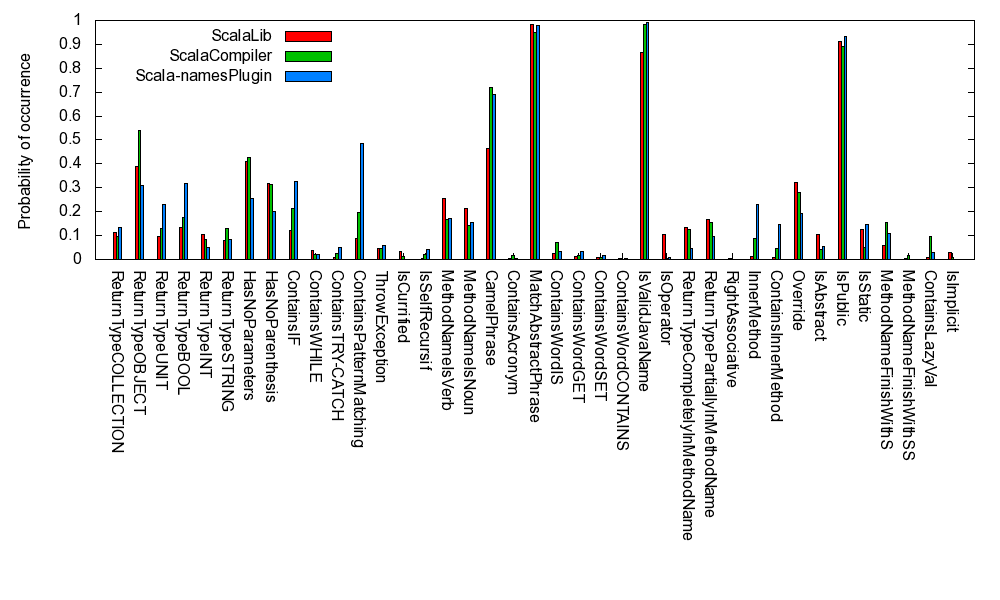
\includegraphics[width=15cm]{images/percent.png}
\caption{Probabilities of occurrence of features.}
\label{fig:features}
\end{figure}
In figure~\ref{fig:features} we can see the probability of occurrence of all 39 features inside the Scala library, the Scala compiler and in my Scala-names plug-in. Note that the package \textit{scala$\backslash$tools$\backslash$ant} of the Scala compiler is not contained inside this analysis. This represent 11'753 method declarations inside the Scala library, 11'730 in the Scala compiler and 199 for the Scala-names plug-in. First of all, we can see in figure~\ref{fig:features} that very few features occur more than 20\%. As they are not frequent we don't obtain a lot of information on them, thus it's hard to find out correct correlation between two features. We can also note that I use a lot more of pattern matching in this project than it's used inside the Scala library or compiler. The library and the compiler also contains less inner methods. We can argue from theses facts that the Scala library and compiler are written in a better functional, Scala-way of coding.
%\begin{enumerate}
%\item Feature~\ref{fCollection} and~\ref{fs} should be correlated as it's a convention that method returning a collection finish with \textit{s}. The correlation matrix in figure~\ref{corrCor} output a 0.8
%\end{enumerate}
\subsubsection {Correlation}
\label{results:corr}
Figures~\ref{corrCor} and~\ref{corrCor2} show the correlation between two features in the Scala library and respectively in the Scala compiler. The coefficient of correlation $c$ between two features is calculated as follow:
\begin{align*}
c &= \frac{a+b}{||m||} :\\ a = \sum i : m_{i_{f_1}}&==1\mbox{ AND }m_{i_{f_2}}==1\\ b = \sum i : m_{i_{f_1}}&==0\mbox{ AND }m_{i_{f_2}}==0
\end{align*}
With $m$ the set of all method declarations, $m_{i_{f_j}}$ the result of the feature $j$ applied to method $m_i$ and $||m||$ the cardinality of $m$.\\
% for every method definitions inside the corpus, for every features two by two, addition the number of time both features are equals and divide the result by the number of method definitions in the corpus.
If two features are often both found or both negative in a single method definition, they have a high correlation coefficient. Note that this does not mean that they are really correlated. By example, if no plane crash today and no nuclear power plant explode today, this doesn't mean that tomorrow if a plane crash, the nearest nuclear power plant will explode. Thanks Philippe for this example.\\

Figures~\ref{corrJac} and~\ref{corrJac2} show the Jaccard coefficient $c_j$. It measures the normalized similarity between two features respectively in the Scala library and in the Scala compiler. It's calculated as follow: 
\begin{align*}
c_j &= \frac{a}{p}:\\ a = \sum i: m_{i_{f_1}}&== 1\mbox{ AND } m_{i_{f_2}}==1\\ p = \sum i : m_{i_{f_1}}&== 1\mbox{ OR }m_{i_{f_2}}==1
\end{align*}
With $m$ the set of all method declarations, $m_{i_{f_j}}$ the result of the feature $j$ applied to method $m_i$. For the Jaccard coefficient matrix, I double the column to add the inverse of all features.\\

Here is a list of observations made on figures~\ref{corrCor} to~\ref{corrJac2}:
%for every method definitions inside the corpus, for every features two by two, addition the number of time both feature are equals to one and divide the result by the amount of methods definitions.
\begin{figure}[h]
\hspace*{-4cm}
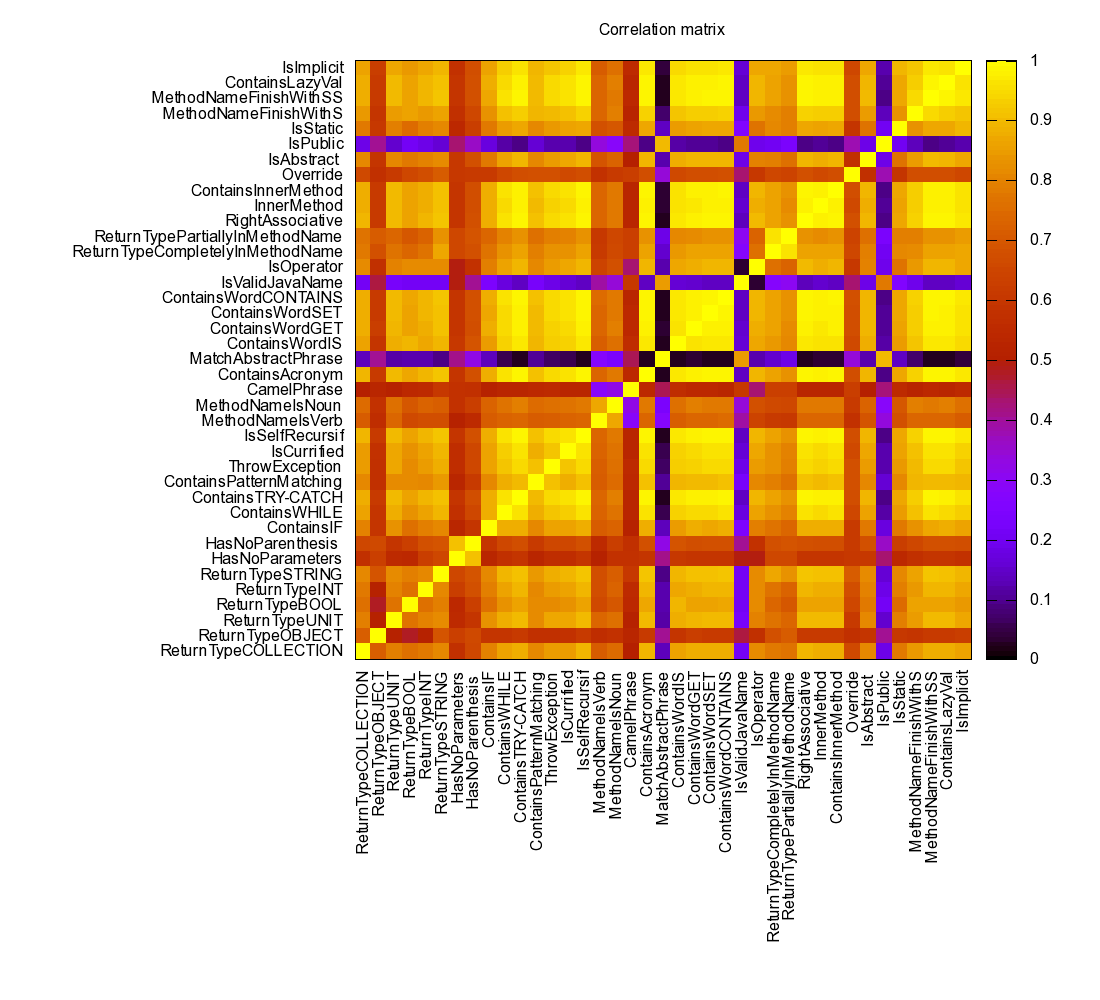
\includegraphics[width=20cm]{images/corrCOR.png}
\caption{Correlation matrix in Scala library}
\label{corrCor}
\end{figure}
\begin{figure}[h]
\hspace*{-3,5cm}
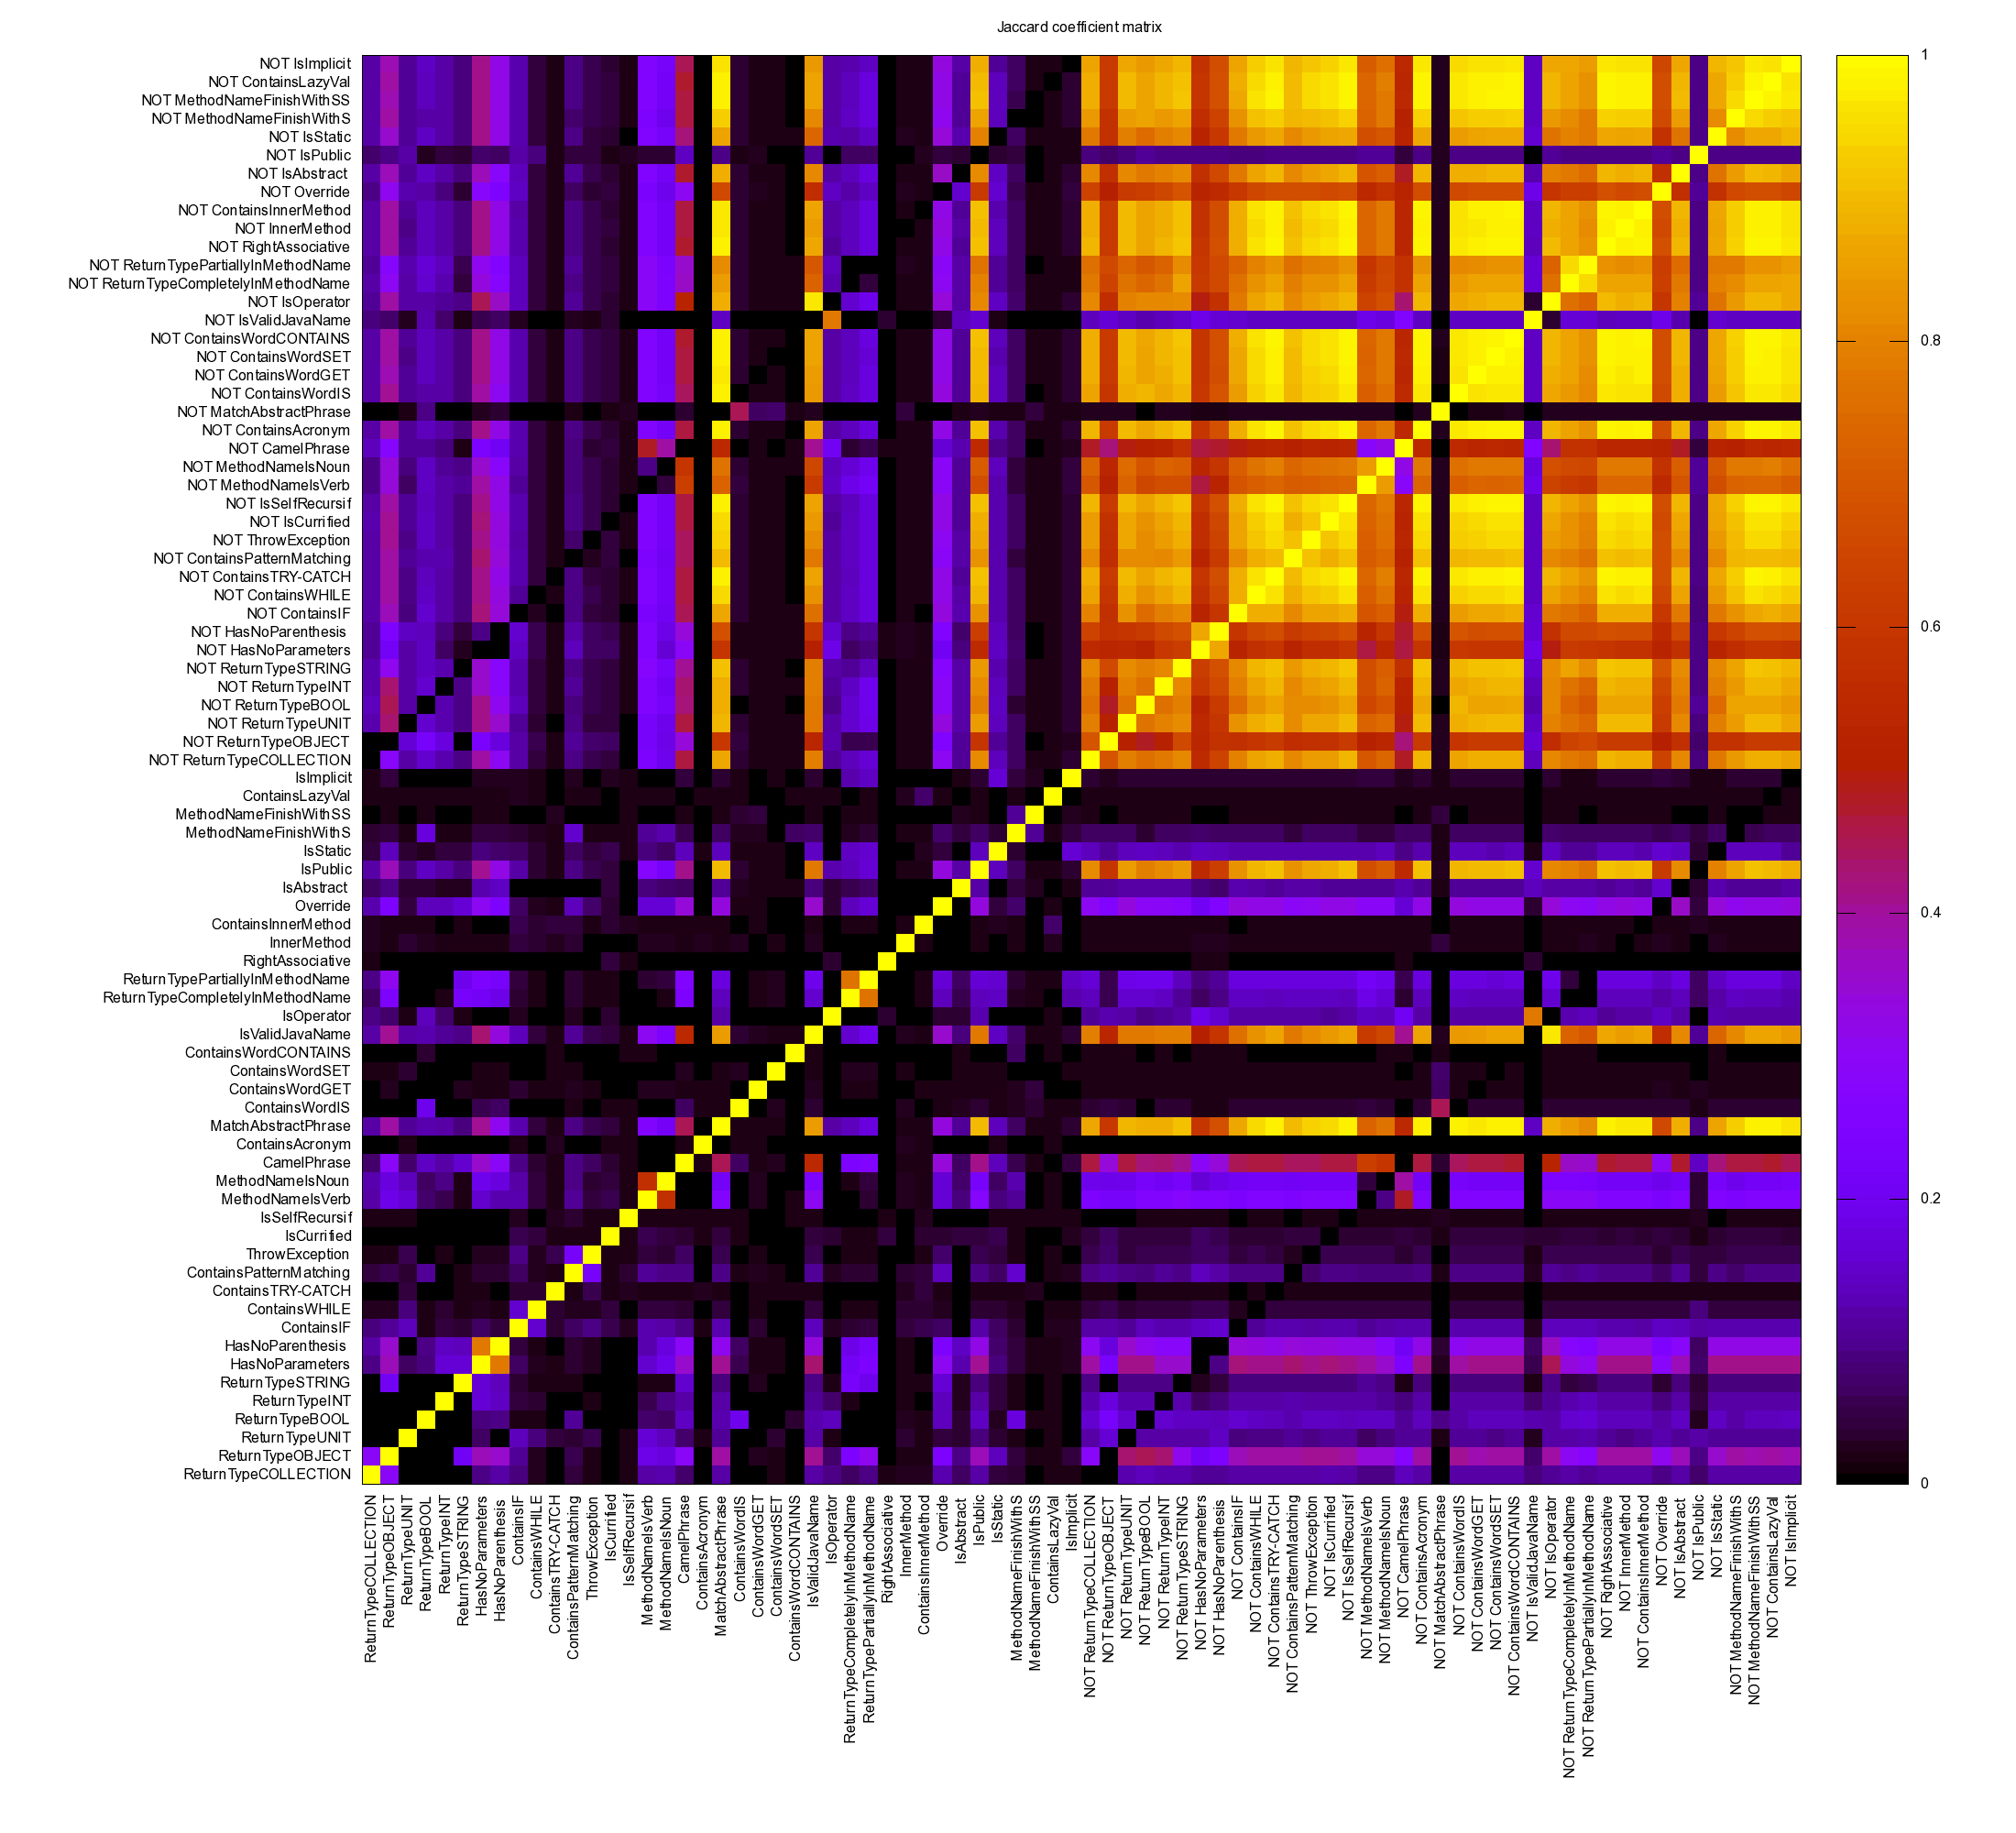
\includegraphics[width=20cm]{images/corrJAC.png}
\caption{Jaccard coefficient matrix in Scala library}
\label{corrJac}
\end{figure}
\begin{figure}[h]
\hspace*{-4cm}
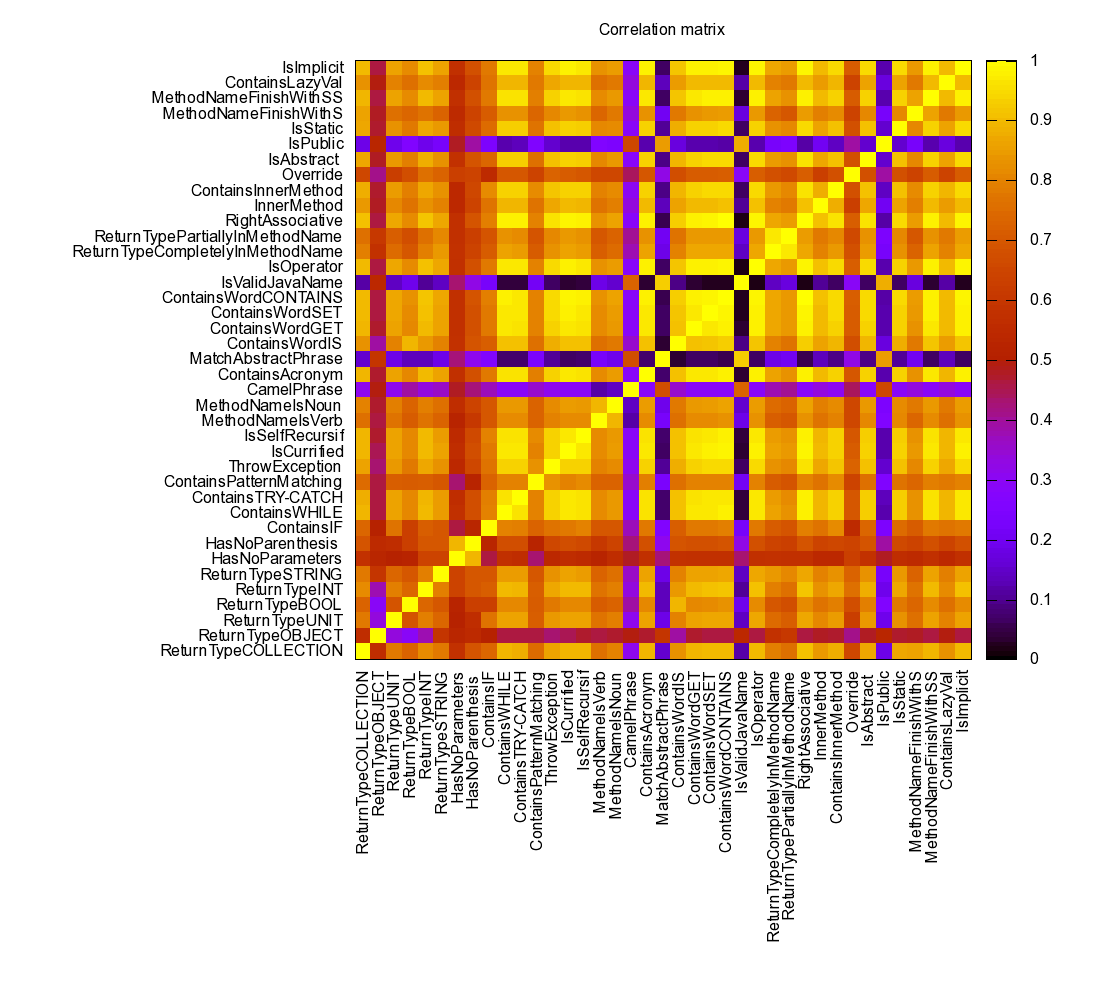
\includegraphics[width=20cm]{images/corrCOR2.png}
\caption{Correlation matrix in Scala compiler}
\label{corrCor2}
\end{figure}
\begin{figure}[h]
\hspace*{-3,5cm}
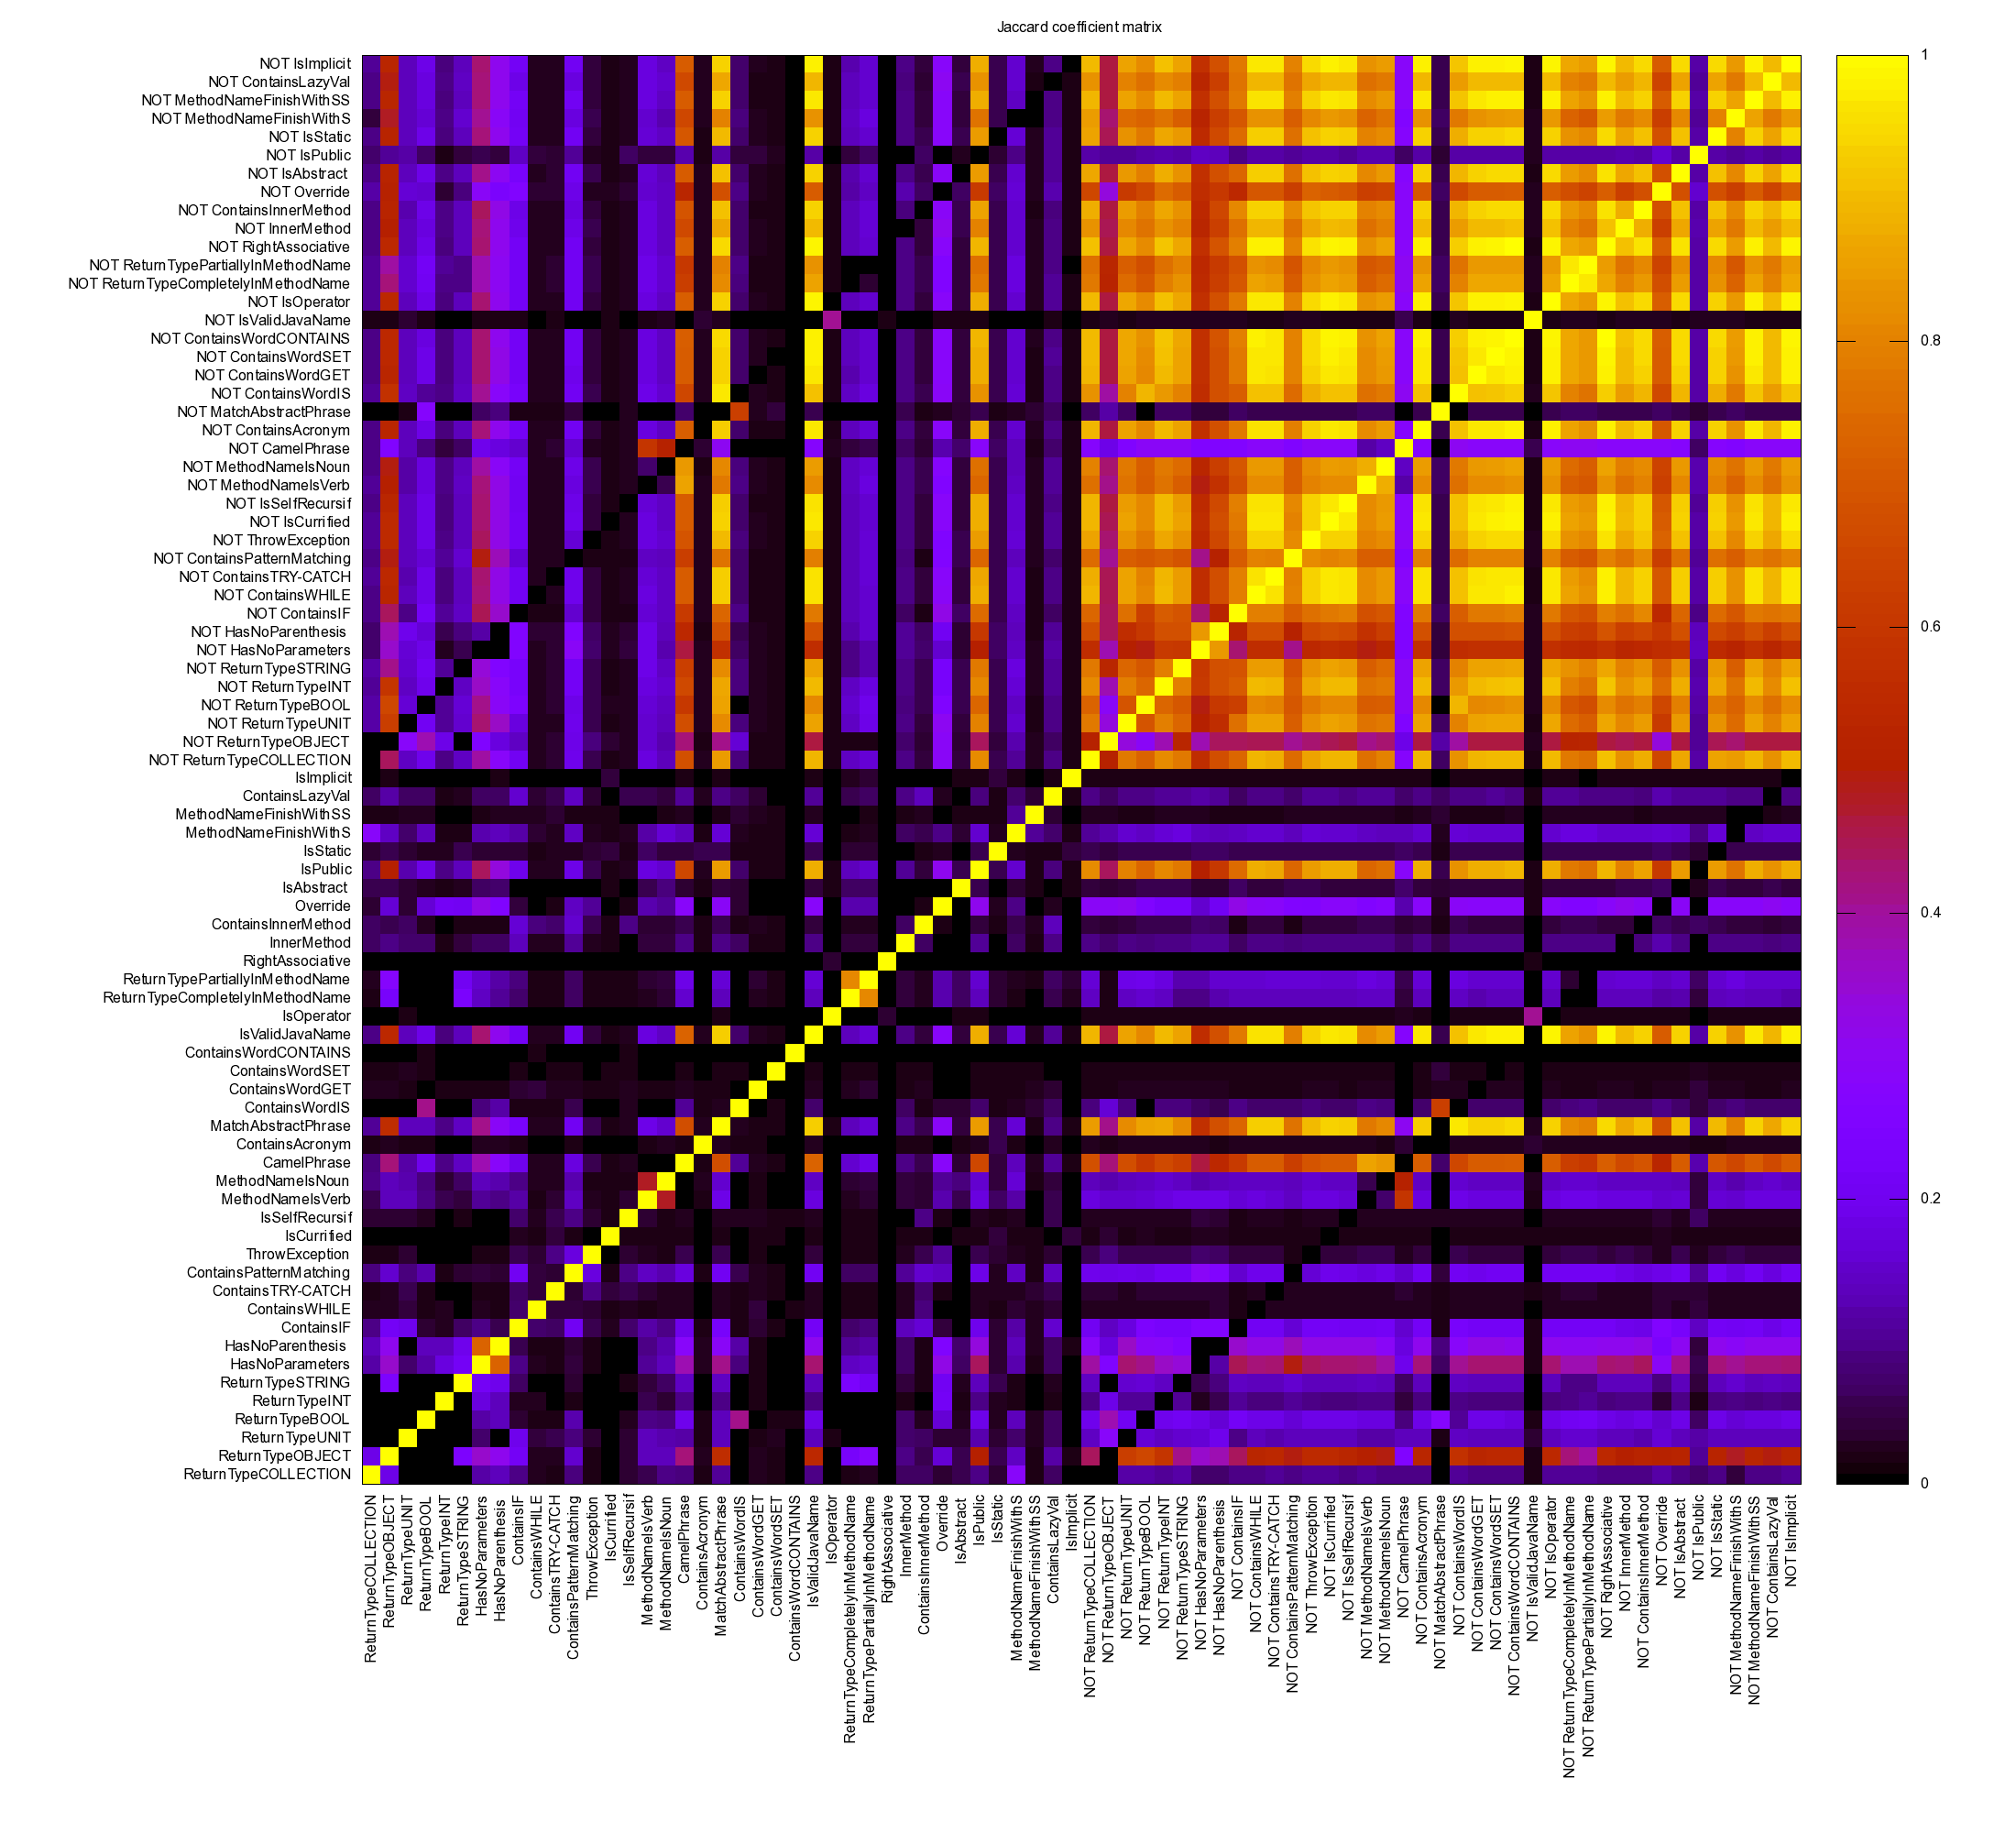
\includegraphics[width=20cm]{images/corrJAC2.png}
\caption{Jaccard coefficient matrix in Scala compiler}
\label{corrJac2}
\end{figure}
\begin{itemize}
\item The first thing we see in correlation matrix of figure~\ref{corrCor} is these three blue-black lines. The three features  at theses lines are the three more likely feature to appear: \ref{fAbstractPhrase} \textit{MatchAbstractPhrase},~\ref{fValidJavaName} \textit{IsValidJavaName} and~\ref{fPublic} \textit{IsPlublic}. As compared to theses, others features appear not so often, their correlation coefficient is really low. We find the opposite pattern, three bright half column in figures~\ref{corrJac} and~\ref{corrJac2} for the same three features. As theses dots are comparing the similarity of features appearing a lot against the inverse of features that appear very few, both are high and thus are similar. But it does not mean, by example, that finding valid Java name exclude a method to contains throw statement.
\item However, there exist an exception to the previous point. Features~\ref{fValidJavaName} \textit{IsValidJavaName} and NOT~\ref{fOperator} \textit{IsOperator} should be similar, which they are. Note the this is not symmetrical. This come from the difference inducted by Java keywords~\cite{jls_keyword}. An example is \textit{break}. It's a valid Scala identifier that is not an operator but is not a valid Java name because it belong to Java keywords.
\item Note the difference of colors between figure~\ref{corrCor} and~\ref{corrCor2}. The correlation matrix of the Scala compiler is slightly darker. This come from the fact that a good number of features are more present in the Scala compiler than in Scala library. We can found out a similar result into figures~\ref{corrJac} and~\ref{corrJac2}.
\FloatBarrier
\item The similarity of features~\ref{fNoParenthesis}, \textit{HasNoParenthesis}, and~\ref{fNoParam}, \textit{HasNoParameter}, is pretty high on both figures~\ref{corrJac} and~\ref{corrJac2}. This is quite normal, as a method without parenthesis should have no parameter.
\item Features based on words \textit{ContainsWordX}~\ref{fContainsIs},~\ref{fContainsGet},~\ref{fContainsSet} and~\ref{fContainsContains} are highly correlated. Of theses features, the~\ref{fContainsIs}, \textit{ContainsWordIS}, is the more present with 2\%, the others are present in less than 1\%. This correlation become from the fact that theses features are very unlikely, they are nearly every times negative and thus are near all the time identical. Note that it's very unlikely that a method name contains both words \textit{set} and \textit{get}. Others features with a probability lower than 1\% obtain a high correlation with theses four features for the same reason. Note that in the correlation matrix of Scala compiler, figure~\ref{corrCor2}, the correlation of feature~\ref{fContainsIs} \textit{ContainsIS} is a bit lower. It's because this feature is more likely to happen, with a 7\%.\\I choose theses four words to be features as they are very often used in Java programming. But it clearly seams it's not the case in Scala. It may be interesting to try a similar feature with \textit{apply}. 
\item The feature~\ref{fss} \textit{MethodNameFinishWithSS}, reveal to be absolutely useless. I checked manually all methods declared inside the Scala library and find out that all methods matching this feature are composed of word that finish with two \textit{s} like: \textit{access}, \textit{success} or \textit{Class}. They are not declared with \textit{ss} because their return type are a collection of collections, but because theses words are written in English with two \textit{s}. I was so disappointed that I didn't even implemented a feature that check a return type of collection of collections, thinking that it would be a waste of time. Note that maybe some methods are actually of this return type and finding that their name do not finish with \textit{ss} would have been an interesting result$\dots$\\
\end{itemize}

\subsection{Analysis}
\label{exp:analysis}
If we assume that the Scala library is well written and consistent, the output of the analysis of the Scala-names plug-in can be useful to find inconsistencies of methods in a given file. Or even naming bugs if an inconsistency rise on a naming property feature. However, one might try on purpose something that violate the Scala conventions or even this person work with different conventions. Outliers can arise inside clustering. Plus, the approximation found by a \textit{k}-means run can be arbitrarily bad with the respect to the objective function compared to the optimal clustering~\cite{kMeans2}. This analysis can be a tool, but should not be believed with closed eyes as the ultimate answer.\\
The \textit{k}-means algorithm output clusters of similar size. But is this a good assumption for clustering method declarations? Based on the Scala library, I think it could be. However I have no proof of this, neither of the opposite. To obtains more details, it would need to be tested with different clustering algorithms.\\
H{\o}st and {\O}stvold used orthogonal features to calculate distance between methods~\cite{DebugMN}. Orthogonal features are features completely independent of each others. A counterexample can be features \textit{ReturnTypeBoolean} and \textit{ReturnTypeString}. If \textit{ReturnTypeBoolean} is true, then off course \textit{ReturnTypeString} will return false. Two similar methods only differentiated by their return type would be in this project at a distance of 2 although they have only one fundamental difference. With these orthogonal features, we might find a better clustering and thus a more relevant analysis.
\section {Conclusion} 
This project has not shown outstanding new results. Nevertheless it confirm some assumptions and Scala language properties. In a way to obtain new results, this project should be extended with more features. The analysis should not only based on method declarations and need to be improved, maybe with orthogonal features or multiple clusterings. The analysis option developed during this project is nice, but is subject to interpretation. Is \textit{k}-means clustering really relevant to find inconsistencies? I think to some points yes, however it should not be believed blindly. It really should be used jointly with others tools.

\section {Future Work}
In this section is listed future work that could improve this project.
\subsection{Adding New Features}
The list of features implemented is off course not exhaustive and can be greatly improved. Here is a list of possible interesting features:
\begin{itemize}
\item The Scala compiler can infer type. So programmers don't need to always specify the return type of a method. In some case the type could be a good indication to the reader to understand the code. But in other case like the method \textit{toString()} we don't really need to see the type written to know its type. Adding a feature returning if the type is declared or inferred, may obtain information about code quality. However, after the \textit{refchecks} phase of the Scala compiler, it's no more possible to obtain the information if the compiler infer the type or if it was declared. It would need another plug-in insert early in the Scala compiler. 
\item A feature matching assignment of variables declared in a larger scope could be used in conjunction with feature~\ref{fNoParenthesis} \textit{NoParenthesis}, to find if the Scala convention is respected or not.
\item As suggested in section~\ref{results:corr} features based on Java words seams not really relevant. Scala words, like \textit{apply}, might give a better results.
\item Scala language contains local import. This can remove ambiguity or add convenient typo to long or frequently used expression. A feature matching these could also find valuable information about code quality. However, declarations of these local imports are already removed of the abstract syntax tree by a previous phase of the compiler. Again, it would need another phase inserted earlier.
\end{itemize}
\subsection{Compose With Others Analysis}
Method names are not the only "objects" that programmers name. They also name variables, class, parameters and types. An analysis of these "objects" can also find out to be interesting. By example, the feature~\ref{fss} \textit{MethodNameFinishWithSS}, give nothing with method name but could highlight something on variables.\\
Cross analysis on all objects can also demonstrate some results.
\subsection{Multiple clusterings}
As stated in~\ref{exp:analysis} the result of \textit{k}-means really depend on the random partitioning. Cluster may be empty, may contains outliers, different runs may put two similar methods in different clusters or output a poor clustering. Currently the analysis of files compared to the library is fixed and based on only one clustering. This is not optimal. Give the possibility to the user to compare against arbitrary corpus and to modify the clustering by a new run of \textit{k}-means or of another clustering algorithm would be a first improvement.\\
A system with multiple clusterings available that the user may select or reject would be less affected by outliers and thus would give a more appropriate result.\\
We could also imagine a system where the user can choose different weights to apply to certain features to guide the clustering.
\newpage
\section{Annexes}
\subsection{Analysis example}
\label{annexe1}
This is an example of the analysis output for one method described in section~\ref{analysis}. When you analyze a file you will get a similar output for every method declarations in that file.\code{
--- Method: splitAt@source-.$\backslash$scala$\backslash$collection$\backslash$immutable$\backslash$List.scala,line-191,offset=6483 ---\\
Sign: 0 1 0 0 0 0 0 0 0 1 0 0 0 0 0 0 0 1 0 1 0 0 0 0 1 0 0 0 0 0 0 1 0 1 0 0 0\\
Nearest cluster: 8 at distance 2.0097560975609756\\
cPos: 0 0 0 ? ? 0 ? 0 0 0 0 ? ? 0 0 0 0 1 0 1 0 0 0 0 1 0 0 0 0 0 0 1 0 1 0 0 0\\
Similar methods:\\
\ \ \ \ \ \ \ \ \ hashCode@source-.$\backslash$scala$\backslash$concurrent$\backslash$pilib.scala,line-127,offset=3904\\
sign: 0 0 0 0 1 0 1 0 0 0 0 0 0 0 0 0 0 1 0 1 0 0 0 0 1 0 0 0 0 0 0 1 0 1 0 0 0\\
\ \ \ \ \ \ \ \ \ canEqual@source-.$\backslash$scala$\backslash$Option.scala,line-261,offset=9053\\
sign: 0 0 0 1 0 0 0 0 0 0 0 0 0 0 0 0 0 1 0 1 0 0 0 0 1 0 0 0 0 0 0 1 0 1 0 0 0\\
\ \ \ \ \ \ \ \ \ productElement@source-.$\backslash$scala$\backslash$reflect$\backslash$generic$\backslash$Trees.scala,line-190,offset=6295\\
sign: 0 0 0 0 0 0 0 0 0 0 0 1 1 0 0 0 0 1 0 1 0 0 0 0 1 0 0 0 0 0 0 1 0 1 0 0 0\\
(\ )(\ )(\ )\ \ \ \=Haz NOT\ \ \ \ \ \ \ \ \ \ \ \ \ \ \ \ \ \ \ \ \ \ \ \ \ \ \ \ \ \=Method returns a collection (Traversable)\\
(\ )(\ )(\ ) \>Haz \ \ \ \ \ \ \ \ BUT should NOT Method returns a subtype of class Object\\
(\ )(\ )(\ ) \>Haz NOT                \>Method return is of type: class Unit\\
(\ )(x)(\ ) \>Haz NOT\ \ \ \ \ \ \ \ \ \ \ \ \ ...       \>Method return is of type: class Boolean\\
(x)(\ )(\ ) \>Haz NOT\ \ \ \ \ \ \ \ \ \ \ \ \ ...       \>Method return is of type: class Int\\
(\ )(\ )(\ ) \>Haz NOT                \>Method return is of type: class String\\
(x)(\ )(\ ) \>Haz NOT\ \ \ \ \ \ \ \ \ \ \ \ \     ...       \>Method have no parameter\\
(\ )(\ )(\ ) \>Haz NOT                \>Method has no parenthesis\\
(\ )(\ )(\ ) \>Haz NOT                \>Method contains IF statement.\\
(\ )(\ )(\ ) \>Haz \ \ \ \ \ \ \ \ BUT should NOT Method contains WHILE statement\\
(\ )(\ )(\ ) \>Haz NOT                \>Method contains TRY/CATCH statement\\
(\ )(\ )(x) \>Haz NOT\ \ \ \ \ \ \ \ \ \ \ \ \ ...       \>Method contains Pattern matching\\
(\ )(\ )(x) \>Haz NOT\ \ \ \ \ \ \ \ \ \ \ \ \ ...       \>Method may explicitly throw an exception\\
(\ )(\ )(\ ) \>Haz NOT                \>Method is currified\\
(\ )(\ )(\ ) \>Haz NOT               \> Method contains a self-recursion\\
(\ )(\ )(\ ) \>Haz NOT               \> MethodName is a verb\\
(\ )(\ )(\ ) \>Haz NOT               \> MethodName is a noun\\
(x)(x)(x) \>Haz  \ \ \ \ \ \ \                    \> MethodName is a camel phrase\\
(\ )(\ )(\ ) \>Haz NOT               \> MethodName contains an acronym\\
(x)(x)(x) \>Haz  \ \ \ \ \ \ \                   \> MethodName match abstract phrase construction\\
(\ )(\ )(\ ) \>Haz NOT               \> MethodName contains "is" pattern\\
(\ )(\ )(\ ) \>Haz NOT                \>MethodName contains "get" pattern\\
(\ )(\ )(\ ) \>Haz NOT               \> MethodName contains "set" pattern\\
(\ )(\ )(\ ) \>Haz NOT              \> MethodName contains "contains" pattern\\
(x)(x)(x) \>Haz  \ \ \ \ \ \ \                   \> MethodName is a valid Java name\\
(\ )(\ )(\ ) \>Haz NOT               \> MethodName is an operator\\
(\ )(\ )(\ ) \>Haz NOT               \> Method return type is completely contained into methodName \\
(\ )(\ )(\ ) \>Haz NOT\>Method return type is partially into the methodName\\
(\ )(\ )(\ ) \>Haz NOT               \> Method is right associative\\
(\ )(\ )(\ ) \>Haz NOT\>Method is defined inside another method\\
(\ )(\ )(\ ) \>Haz NOT               \> Method body contains method definition\\
(x)(x)(x) \>Haz  \ \ \ \ \ \ \           \>        Method is overriding another method\\
(\ )(\ )(\ ) \>Haz NOT        \>       Method is abstract\\
(x)(x)(x) \>Haz  \ \ \ \ \ \ \            \>        Method is public\\
(\ )(\ )(\ ) \>Haz NOT             \>   Method is static\\
(\ )(\ )(\ ) \>Haz NOT\>Method finish with s\\
(\ )(\ )(\ ) \>Haz NOT           \>     Method finish with ss}


\newpage

\bibliographystyle{plain}
\bibliography{EricZbinden_ScalaNames}

\end{document}